\documentclass[]{report}
\usepackage{lmodern}
\usepackage{amssymb,amsmath}
\usepackage{ifxetex,ifluatex}
\usepackage{fixltx2e} % provides \textsubscript
\ifnum 0\ifxetex 1\fi\ifluatex 1\fi=0 % if pdftex
  \usepackage[T1]{fontenc}
  \usepackage[utf8]{inputenc}
\else % if luatex or xelatex
  \ifxetex
    \usepackage{mathspec}
  \else
    \usepackage{fontspec}
  \fi
  \defaultfontfeatures{Ligatures=TeX,Scale=MatchLowercase}
\fi
% use upquote if available, for straight quotes in verbatim environments
\IfFileExists{upquote.sty}{\usepackage{upquote}}{}
% use microtype if available
\IfFileExists{microtype.sty}{%
\usepackage{microtype}
\UseMicrotypeSet[protrusion]{basicmath} % disable protrusion for tt fonts
}{}
\usepackage{hyperref}
\hypersetup{unicode=true,
            pdftitle={Project 2 - Group 2 Homework Part 2},
            pdfauthor={Vinicio Haro; Sang Yoon (Andy) Hwang; Julian McEachern; Jeremy O'Brien; Bethany Poulin},
            pdfborder={0 0 0},
            breaklinks=true}
\urlstyle{same}  % don't use monospace font for urls
\usepackage{color}
\usepackage{fancyvrb}
\newcommand{\VerbBar}{|}
\newcommand{\VERB}{\Verb[commandchars=\\\{\}]}
\DefineVerbatimEnvironment{Highlighting}{Verbatim}{commandchars=\\\{\}}
% Add ',fontsize=\small' for more characters per line
\usepackage{framed}
\definecolor{shadecolor}{RGB}{248,248,248}
\newenvironment{Shaded}{\begin{snugshade}}{\end{snugshade}}
\newcommand{\AlertTok}[1]{\textcolor[rgb]{0.94,0.16,0.16}{#1}}
\newcommand{\AnnotationTok}[1]{\textcolor[rgb]{0.56,0.35,0.01}{\textbf{\textit{#1}}}}
\newcommand{\AttributeTok}[1]{\textcolor[rgb]{0.77,0.63,0.00}{#1}}
\newcommand{\BaseNTok}[1]{\textcolor[rgb]{0.00,0.00,0.81}{#1}}
\newcommand{\BuiltInTok}[1]{#1}
\newcommand{\CharTok}[1]{\textcolor[rgb]{0.31,0.60,0.02}{#1}}
\newcommand{\CommentTok}[1]{\textcolor[rgb]{0.56,0.35,0.01}{\textit{#1}}}
\newcommand{\CommentVarTok}[1]{\textcolor[rgb]{0.56,0.35,0.01}{\textbf{\textit{#1}}}}
\newcommand{\ConstantTok}[1]{\textcolor[rgb]{0.00,0.00,0.00}{#1}}
\newcommand{\ControlFlowTok}[1]{\textcolor[rgb]{0.13,0.29,0.53}{\textbf{#1}}}
\newcommand{\DataTypeTok}[1]{\textcolor[rgb]{0.13,0.29,0.53}{#1}}
\newcommand{\DecValTok}[1]{\textcolor[rgb]{0.00,0.00,0.81}{#1}}
\newcommand{\DocumentationTok}[1]{\textcolor[rgb]{0.56,0.35,0.01}{\textbf{\textit{#1}}}}
\newcommand{\ErrorTok}[1]{\textcolor[rgb]{0.64,0.00,0.00}{\textbf{#1}}}
\newcommand{\ExtensionTok}[1]{#1}
\newcommand{\FloatTok}[1]{\textcolor[rgb]{0.00,0.00,0.81}{#1}}
\newcommand{\FunctionTok}[1]{\textcolor[rgb]{0.00,0.00,0.00}{#1}}
\newcommand{\ImportTok}[1]{#1}
\newcommand{\InformationTok}[1]{\textcolor[rgb]{0.56,0.35,0.01}{\textbf{\textit{#1}}}}
\newcommand{\KeywordTok}[1]{\textcolor[rgb]{0.13,0.29,0.53}{\textbf{#1}}}
\newcommand{\NormalTok}[1]{#1}
\newcommand{\OperatorTok}[1]{\textcolor[rgb]{0.81,0.36,0.00}{\textbf{#1}}}
\newcommand{\OtherTok}[1]{\textcolor[rgb]{0.56,0.35,0.01}{#1}}
\newcommand{\PreprocessorTok}[1]{\textcolor[rgb]{0.56,0.35,0.01}{\textit{#1}}}
\newcommand{\RegionMarkerTok}[1]{#1}
\newcommand{\SpecialCharTok}[1]{\textcolor[rgb]{0.00,0.00,0.00}{#1}}
\newcommand{\SpecialStringTok}[1]{\textcolor[rgb]{0.31,0.60,0.02}{#1}}
\newcommand{\StringTok}[1]{\textcolor[rgb]{0.31,0.60,0.02}{#1}}
\newcommand{\VariableTok}[1]{\textcolor[rgb]{0.00,0.00,0.00}{#1}}
\newcommand{\VerbatimStringTok}[1]{\textcolor[rgb]{0.31,0.60,0.02}{#1}}
\newcommand{\WarningTok}[1]{\textcolor[rgb]{0.56,0.35,0.01}{\textbf{\textit{#1}}}}
\usepackage{graphicx,grffile}
\makeatletter
\def\maxwidth{\ifdim\Gin@nat@width>\linewidth\linewidth\else\Gin@nat@width\fi}
\def\maxheight{\ifdim\Gin@nat@height>\textheight\textheight\else\Gin@nat@height\fi}
\makeatother
% Scale images if necessary, so that they will not overflow the page
% margins by default, and it is still possible to overwrite the defaults
% using explicit options in \includegraphics[width, height, ...]{}
\setkeys{Gin}{width=\maxwidth,height=\maxheight,keepaspectratio}
\IfFileExists{parskip.sty}{%
\usepackage{parskip}
}{% else
\setlength{\parindent}{0pt}
\setlength{\parskip}{6pt plus 2pt minus 1pt}
}
\setlength{\emergencystretch}{3em}  % prevent overfull lines
\providecommand{\tightlist}{%
  \setlength{\itemsep}{0pt}\setlength{\parskip}{0pt}}
\setcounter{secnumdepth}{0}

%%% Use protect on footnotes to avoid problems with footnotes in titles
\let\rmarkdownfootnote\footnote%
\def\footnote{\protect\rmarkdownfootnote}

%%% Change title format to be more compact
\usepackage{titling}

% Create subtitle command for use in maketitle
\providecommand{\subtitle}[1]{
  \posttitle{
    \begin{center}\large#1\end{center}
    }
}

\setlength{\droptitle}{-2em}

  \title{Project 2 - Group 2\\
Homework Part 2}
    \pretitle{\vspace{\droptitle}\centering\huge}
  \posttitle{\par}
    \author{Vinicio Haro \\ Sang Yoon (Andy) Hwang \\ Julian McEachern \\ Jeremy O'Brien \\ Bethany Poulin}
    \preauthor{\centering\large\emph}
  \postauthor{\par}
      \predate{\centering\large\emph}
  \postdate{\par}
    \date{10 December 2019}

% set plain style for page numbers
\usepackage[margin=1in]{geometry}
\usepackage{fancyhdr}
\pagestyle{fancy}
\fancyhead[LE,RO]{\textbf{Group 2}}
\fancyhead[RE,LO]{\textbf{Project 2: Predicting PH}}
\raggedbottom
\setlength{\parskip}{1em}

% change font
\usepackage{fontspec}
\setmainfont{Arial}

% format titles 
\usepackage{xcolor}
\usepackage{sectsty}
\usepackage{etoolbox}
\usepackage{titling}
\definecolor{prettyblue}{RGB}{84, 144, 240}
\definecolor{bluegray}{RGB}{98, 107, 115}
\pretitle{\begin{center}\Huge\color{prettyblue}\textbf}
\posttitle{\par\LARGE\color{gray}DATA 624 - Predictive Analytics\linebreak Group 2\end{center}}
\preauthor{\begin{center}\large\textbf{Group Members:}\linebreak\textit}
\postauthor{\end{center}}

% Format chapter output
\usepackage{titlesec}
\titleclass{\part}{top}
\titleclass{\chapter}{straight}
\titleformat{\chapter}
  {\normalfont\color{prettyblue}\LARGE\bfseries}{\thechapter}{1em}{}
\titlespacing*{\chapter}{0pt}{3.5ex plus 1ex minus .2ex}{2.3ex plus .2ex}


% create color block quotes
\usepackage{tcolorbox}
\newtcolorbox{myquote}{colback=purple!05!white, colframe=purple!75!black}
\renewenvironment{quote}{\begin{myquote}}{\end{myquote}}

% kable 
\usepackage{tabu}


% multicolumn
\usepackage{multicol}

% bullets
\newenvironment{tight_enumerate}{
\begin{enumerate}
  \setlength{\itemsep}{0pt}
  \setlength{\parskip}{0pt}
  }{\end{enumerate}}
  
\newenvironment{tight_itemize}{
\begin{itemize}
  \setlength{\topsep}{0pt}
  \setlength{\itemsep}{0pt}
  \setlength{\parskip}{0pt}
  \setlength{\parsep}{0pt}
  }{\end{itemize}}

\usepackage{paralist}

%hyperlink
\usepackage{hyperref}
\hypersetup{
    colorlinks=true,
    linkcolor=bluegray,
    filecolor=magenta,      
    urlcolor=cyan}

\usepackage{graphicx}
\usepackage{wrapfig}
\usepackage{booktabs}
\definecolor{yale}{RGB}{13,77,146}
\usepackage[font={color=yale,bf,scriptsize},figurename=Fig.,belowskip=0pt,aboveskip=0pt]{caption}
\usepackage{floatrow}
\floatsetup[figure]{capposition=above}
\floatsetup[table]{capposition=above}
\setlength{\abovecaptionskip}{1pt}
\setlength{\belowcaptionskip}{1pt}
\setlength{\textfloatsep}{2pt plus 0.5pt minus 0.5pt}
\setlength{\intextsep}{2pt plus 0.5pt minus 0.5pt}
\usepackage{booktabs}
\usepackage{longtable}
\usepackage{array}
\usepackage{multirow}
\usepackage{wrapfig}
\usepackage{float}
\usepackage{colortbl}
\usepackage{pdflscape}
\usepackage{tabu}
\usepackage{threeparttable}
\usepackage{threeparttablex}
\usepackage[normalem]{ulem}
\usepackage{makecell}
\usepackage{xcolor}

\begin{document}
\maketitle

{
\setcounter{tocdepth}{2}
\tableofcontents
}
\hypertarget{Overview}{%
\chapter*{Getting Started}\label{Overview}}
\addcontentsline{toc}{chapter}{Getting Started}

\hypertarget{overview}{%
\section{Overview}\label{overview}}

Include details on our process in creating this document.

\hypertarget{dependencies}{%
\section{Dependencies}\label{dependencies}}

\begin{Shaded}
\begin{Highlighting}[]
\CommentTok{# Predicitve Modeling}
\KeywordTok{libraries}\NormalTok{(}\StringTok{"AppliedPredictiveModeling"}\NormalTok{, }\StringTok{"mice"}\NormalTok{, }\StringTok{"caret"}\NormalTok{, }\StringTok{"tidyverse"}\NormalTok{, }
    \StringTok{"impute"}\NormalTok{, }\StringTok{"pls"}\NormalTok{, }\StringTok{"caTools"}\NormalTok{, }\StringTok{"mlbench"}\NormalTok{, }\StringTok{"car"}\NormalTok{, }\StringTok{"olsrr"}\NormalTok{, }\StringTok{"neuralnet"}\NormalTok{, }
    \StringTok{"nnet"}\NormalTok{, }\StringTok{"earth"}\NormalTok{)}
\CommentTok{# Formatting Libraries}
\KeywordTok{libraries}\NormalTok{(}\StringTok{"default"}\NormalTok{, }\StringTok{"knitr"}\NormalTok{, }\StringTok{"kableExtra"}\NormalTok{, }\StringTok{"readxl"}\NormalTok{, }\StringTok{"sqldf"}\NormalTok{, }
    \StringTok{"sjPlot"}\NormalTok{, }\StringTok{"sjmisc"}\NormalTok{, }\StringTok{"sjlabelled"}\NormalTok{, }\StringTok{"MASS"}\NormalTok{)}
\CommentTok{# Plotting Libraries}
\KeywordTok{libraries}\NormalTok{(}\StringTok{"ggplot2"}\NormalTok{, }\StringTok{"grid"}\NormalTok{, }\StringTok{"ggfortify"}\NormalTok{, }\StringTok{"DataExplorer"}\NormalTok{, }\StringTok{"ggcorrplot"}\NormalTok{)}
\end{Highlighting}
\end{Shaded}

\newpage

\hypertarget{AS-1}{%
\chapter*{Project 2}\label{AS-1}}
\addcontentsline{toc}{chapter}{Project 2}

\textbackslash begin\{question\}\{Project \#2 - Requirement\}You are
given a simple data set from a beverage manufacturing company. It
consists of 2,571 rows/cases of data and 33 columns / variables. Your
goal is to use this data to predict PH (a column in the set). PH is a
measure of acidity/alkalinity, it must conform in a critical range and
therefore it is important to understand its influence and predict its
values. This is production data. PH is a KPI, Key Performance Indicator.

You are also given a scoring set (267 cases). All variables other than
the dependent or target. You will use this data to score your model with
your best predictions. :\textbackslash end\{question\}

\begin{Shaded}
\begin{Highlighting}[]
\NormalTok{df <-}\StringTok{ }\KeywordTok{read_excel}\NormalTok{(}\StringTok{"C:/Users/traveler/Documents/GitHub/CUNY_DATA_624/Project_Two/data/StudentData.xlsx"}\NormalTok{)}
\CommentTok{# df <-}
\CommentTok{# read_excel('~/GitHub/CUNY_DATA_624/Project_Two/data/StudentData.xlsx')}
\NormalTok{df_eval <-}\StringTok{ }\KeywordTok{read_excel}\NormalTok{(}\StringTok{"C:/Users/traveler/Documents/GitHub/CUNY_DATA_624/Project_Two/data/StudentEvaluation.xlsx"}\NormalTok{)}
\CommentTok{# df_eval <-}
\CommentTok{# read_excel('~/GitHub/CUNY_DATA_624/Project_Two/data/StudentEvaluation.xlsx')}
\NormalTok{dict <-}\StringTok{ }\KeywordTok{read_excel}\NormalTok{(}\StringTok{"C:/Users/traveler/Documents/GitHub/CUNY_DATA_624/Project_Two/data/DataDictionary.xlsx"}\NormalTok{)}
\CommentTok{# dict <-}
\CommentTok{# read_excel('~/GitHub/CUNY_DATA_624/Project_Two/data/DataDictionary.xlsx')}
\CommentTok{# remove space in-between variable names}
\KeywordTok{colnames}\NormalTok{(df) <-}\StringTok{ }\KeywordTok{gsub}\NormalTok{(}\StringTok{" "}\NormalTok{, }\StringTok{""}\NormalTok{, }\KeywordTok{colnames}\NormalTok{(df))}
\end{Highlighting}
\end{Shaded}

\newpage
\clearpage
\pagenumbering{arabic}

\hypertarget{intro}{%
\chapter*{Introduction}\label{intro}}
\addcontentsline{toc}{chapter}{Introduction}

The goal of this project is to predict \texttt{PH}, a measure of
acidity/alkalinity, using train data set from a beverage company which
consists of 2571 rows of data and 33 variables. After creating models
based on training data, we will test on scoring set of 267 rows with 32
variables (excluding target variable which is \texttt{PH} in our
training set)

As a group project, each member of the group is responsible for creating
their own models of choice. For instance, my own selections were
\texttt{Linear\ model} and \texttt{NNet}. However, the choice of models
can be altered after careful review of data exploration - it may require
different type of model in case data suffers from outliers or any other
data related issues.

Explaining why some necessary steps were applied before modeling and
model A was preferred to Model B is often a topic in academic papers
which is a meaningful topic that helps audience learn the concept of
bagged regression and least square method better.

The final version of report will contain all of our approaches with
results of \texttt{MAPE} for each model with detailed explanation of
why/what/how each model of choice was chosen.

NNet, linear model, and one of your choice

\newpage

\hypertarget{data-exploration}{%
\chapter{Data Exploration}\label{data-exploration}}

\hypertarget{data-dictionary}{%
\section{Data dictionary}\label{data-dictionary}}

The table below describes the variables in the train data set.

\begin{Shaded}
\begin{Highlighting}[]
\KeywordTok{kable}\NormalTok{(dict, }\DataTypeTok{caption =} \StringTok{"Data dictionary"}\NormalTok{, }\DataTypeTok{booktabs =}\NormalTok{ T) }\OperatorTok\StringTok{ }\KeywordTok{kable_styling}\NormalTok{() }\OperatorTok\StringTok{ }
\StringTok{    }\KeywordTok{row_spec}\NormalTok{()}
\end{Highlighting}
\end{Shaded}

\begin{table}[H]

\caption{\label{tab:project2a1}Data dictionary}
\centering
\begin{tabular}[t]{llrrll}
\toprule
\textbf{Name} & \textbf{Type} & \textbf{MD code} & \textbf{Length} & \textbf{Measurement Type} & \textbf{Excluded}\\
\midrule
\rowcolor{gray!6}  Test Time & Double & -9999 & 8 & m/d/yy h:mm Am/Pm & Auto\\
Brand Code & Double & -9999 & 8 & General & Categorical\\
\rowcolor{gray!6}  Carb Volume & Double & -9999 & 8 & General & Auto\\
Fill Ounces & Double & -9999 & 8 & General & Auto\\
\rowcolor{gray!6}  PC Volume & Double & -9999 & 8 & General & Auto\\
\addlinespace
Carb Pressure & Double & -9999 & 8 & General & Auto\\
\rowcolor{gray!6}  Carb Temp & Double & -9999 & 8 & General & Auto\\
PSC & Double & -9999 & 8 & General & Auto\\
\rowcolor{gray!6}  PSC Fill & Double & -9999 & 8 & General & Auto\\
PSC CO2 & Double & -9999 & 8 & General & Auto\\
\addlinespace
\rowcolor{gray!6}  Mnf Flow & Double & -9999 & 8 & General & Auto\\
Carb Pressure1 & Double & -9999 & 8 & General & Auto\\
\rowcolor{gray!6}  Fill Pressure & Double & -9999 & 8 & General & Auto\\
Hyd Pressure1 & Double & -9999 & 8 & General & Auto\\
\rowcolor{gray!6}  Hyd Pressure2 & Double & -9999 & 8 & General & Auto\\
\addlinespace
Hyd Pressure3 & Double & -9999 & 8 & General & Auto\\
\rowcolor{gray!6}  Hyd Pressure4 & Double & -9999 & 8 & General & Auto\\
Filler Level & Double & -9999 & 8 & General & Auto\\
\rowcolor{gray!6}  Filler Speed & Double & -9999 & 8 & General & Auto\\
Temperature & Double & -9999 & 8 & General & Auto\\
\addlinespace
\rowcolor{gray!6}  Usage cont & Double & -9999 & 8 & General & Auto\\
Carb Flow & Double & -9999 & 8 & General & Auto\\
\rowcolor{gray!6}  Density & Double & -9999 & 8 & General & Auto\\
MFR & Double & -9999 & 8 & General & Auto\\
\rowcolor{gray!6}  Balling & Double & -9999 & 8 & General & Auto\\
\addlinespace
Pressure Vacuum & Double & -9999 & 8 & General & Auto\\
\rowcolor{gray!6}  PH & Double & -9999 & 8 & General & Auto\\
Oxygen Filler & Double & -9999 & 8 & General & Auto\\
\rowcolor{gray!6}  Bowl Setpoint & Double & -9999 & 8 & General & Auto\\
Pressure Setpoint & Double & -9999 & 8 & General & Auto\\
\addlinespace
\rowcolor{gray!6}  Air Pressurer & Double & -9999 & 8 & General & Auto\\
Alch Rel & Double & -9999 & 8 & General & Auto\\
\rowcolor{gray!6}  Carb Rel & Double & -9999 & 8 & General & Auto\\
Balling Lvl & Double & -9999 & 8 & General & Auto\\
\rowcolor{gray!6}  sample & Double & -999999998 & 8 & General & Auto\\
\bottomrule
\end{tabular}
\end{table}

\newpage

Before we begin to try models against our data, we need to get an
understanding of what our data looks like. We want to know what
variables contain missing data. We also want to see the distributions of
our target variable in addition to predictors. We need to establish a
direction when it comes to pre-processing methods such as imputation,
variable removal, and transformations. As a first step, we want to see
the percentage of missing data per variable.

\begin{Shaded}
\begin{Highlighting}[]
\CommentTok{# code}
\KeywordTok{round}\NormalTok{((}\KeywordTok{apply}\NormalTok{(df, }\DecValTok{2}\NormalTok{, }\ControlFlowTok{function}\NormalTok{(col) }\KeywordTok{sum}\NormalTok{(}\KeywordTok{is.na}\NormalTok{(col))}\OperatorTok{/}\KeywordTok{length}\NormalTok{(col))) }\OperatorTok{*}\StringTok{ }
\StringTok{    }\DecValTok{100}\NormalTok{, }\DecValTok{2}\NormalTok{) }\OperatorTok\StringTok{ }\KeywordTok{kable}\NormalTok{(}\DataTypeTok{caption =} \StringTok{"Distribution of Missing data in Beverage Manufacturing Company Data"}\NormalTok{) }\OperatorTok\StringTok{ }
\StringTok{    }\KeywordTok{kable_styling}\NormalTok{(}\DataTypeTok{full_width =}\NormalTok{ F, }\DataTypeTok{position =} \StringTok{"center"}\NormalTok{) }\OperatorTok\StringTok{ }\KeywordTok{row_spec}\NormalTok{()}
\end{Highlighting}
\end{Shaded}

\begin{table}[H]

\caption{\label{tab:project2a2}Distribution of Missing data in Beverage Manufacturing Company Data}
\centering
\begin{tabular}[t]{l|r}
\hline
\textbf{ } & \textbf{x}\\
\hline
\rowcolor{gray!6}  BrandCode & 4.67\\
\hline
CarbVolume & 0.39\\
\hline
\rowcolor{gray!6}  FillOunces & 1.48\\
\hline
PCVolume & 1.52\\
\hline
\rowcolor{gray!6}  CarbPressure & 1.05\\
\hline
CarbTemp & 1.01\\
\hline
\rowcolor{gray!6}  PSC & 1.28\\
\hline
PSCFill & 0.89\\
\hline
\rowcolor{gray!6}  PSCCO2 & 1.52\\
\hline
MnfFlow & 0.08\\
\hline
\rowcolor{gray!6}  CarbPressure1 & 1.24\\
\hline
FillPressure & 0.86\\
\hline
\rowcolor{gray!6}  HydPressure1 & 0.43\\
\hline
HydPressure2 & 0.58\\
\hline
\rowcolor{gray!6}  HydPressure3 & 0.58\\
\hline
HydPressure4 & 1.17\\
\hline
\rowcolor{gray!6}  FillerLevel & 0.78\\
\hline
FillerSpeed & 2.22\\
\hline
\rowcolor{gray!6}  Temperature & 0.54\\
\hline
Usagecont & 0.19\\
\hline
\rowcolor{gray!6}  CarbFlow & 0.08\\
\hline
Density & 0.04\\
\hline
\rowcolor{gray!6}  MFR & 8.25\\
\hline
Balling & 0.04\\
\hline
\rowcolor{gray!6}  PressureVacuum & 0.00\\
\hline
PH & 0.16\\
\hline
\rowcolor{gray!6}  OxygenFiller & 0.47\\
\hline
BowlSetpoint & 0.08\\
\hline
\rowcolor{gray!6}  PressureSetpoint & 0.47\\
\hline
AirPressurer & 0.00\\
\hline
\rowcolor{gray!6}  AlchRel & 0.35\\
\hline
CarbRel & 0.39\\
\hline
\rowcolor{gray!6}  BallingLvl & 0.04\\
\hline
\end{tabular}
\end{table}

MFR is missing 8.25\% of its data followed by BrandCode,which is missing
a little under 5\% of its data. Brandcode isa categorical variable. The
rest of our predictors are missing less than 3\% of their data if not
missing any at all. We can deal with these variables using a method of
imputation. From our previous experience, we have used MICE succesfully
as an imputation method. We have previously found that there does not
seem to be major changes in the summary statistics across different
imputation methods such as KNN or mean/mode. We also see that we are
missing a small amount of data in the target variable (PH). PH is our
ground truth, therefore it is better to remove rows where ground truth
is missing without major data loss. We next examine the distribution of
our response and predictor variables.

\begin{Shaded}
\begin{Highlighting}[]
\CommentTok{# drop rows where PH is missing}
\NormalTok{df <-}\StringTok{ }\KeywordTok{sqldf}\NormalTok{(}\StringTok{"select}
\StringTok{*}
\StringTok{from df}
\StringTok{where PH is not null}
\StringTok{      "}\NormalTok{)}


\NormalTok{df }\OperatorTok\StringTok{ }\KeywordTok{ggplot}\NormalTok{(}\KeywordTok{aes}\NormalTok{(PH)) }\OperatorTok{+}\StringTok{ }\KeywordTok{geom_histogram}\NormalTok{(}\DataTypeTok{bins =} \DecValTok{30}\NormalTok{) }\OperatorTok{+}\StringTok{ }\KeywordTok{theme_bw}\NormalTok{() }\OperatorTok{+}\StringTok{ }
\StringTok{    }\KeywordTok{theme}\NormalTok{(}\DataTypeTok{legend.position =} \StringTok{"center"}\NormalTok{) }\OperatorTok{+}\StringTok{ }\KeywordTok{labs}\NormalTok{(}\DataTypeTok{y =} \StringTok{"Count"}\NormalTok{, }\DataTypeTok{title =} \StringTok{"Distribution of PH"}\NormalTok{)}
\end{Highlighting}
\end{Shaded}

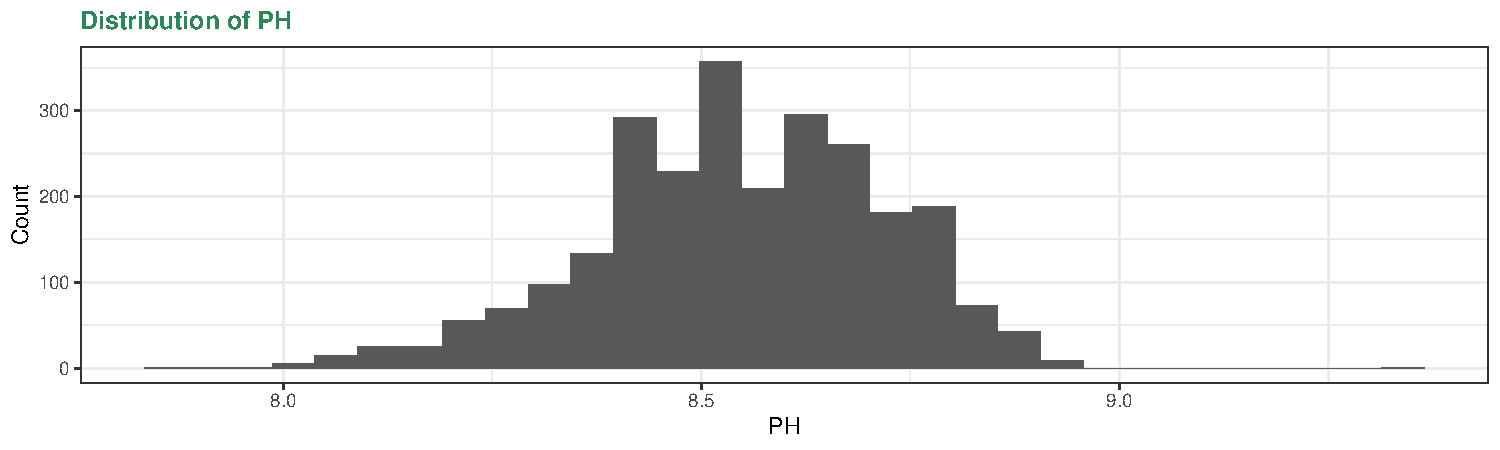
\includegraphics{Project2-VH_files/figure-latex/project2a3-1.pdf}

\begin{Shaded}
\begin{Highlighting}[]
\KeywordTok{plot_histogram}\NormalTok{(df)}
\end{Highlighting}
\end{Shaded}

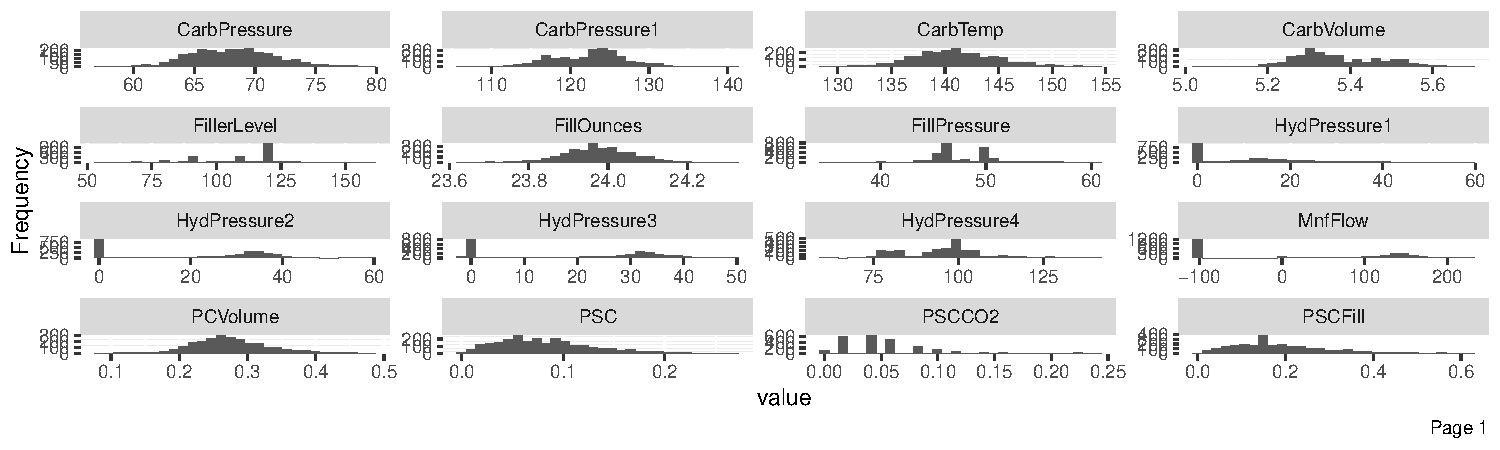
\includegraphics{Project2-VH_files/figure-latex/project2a4-1.pdf}
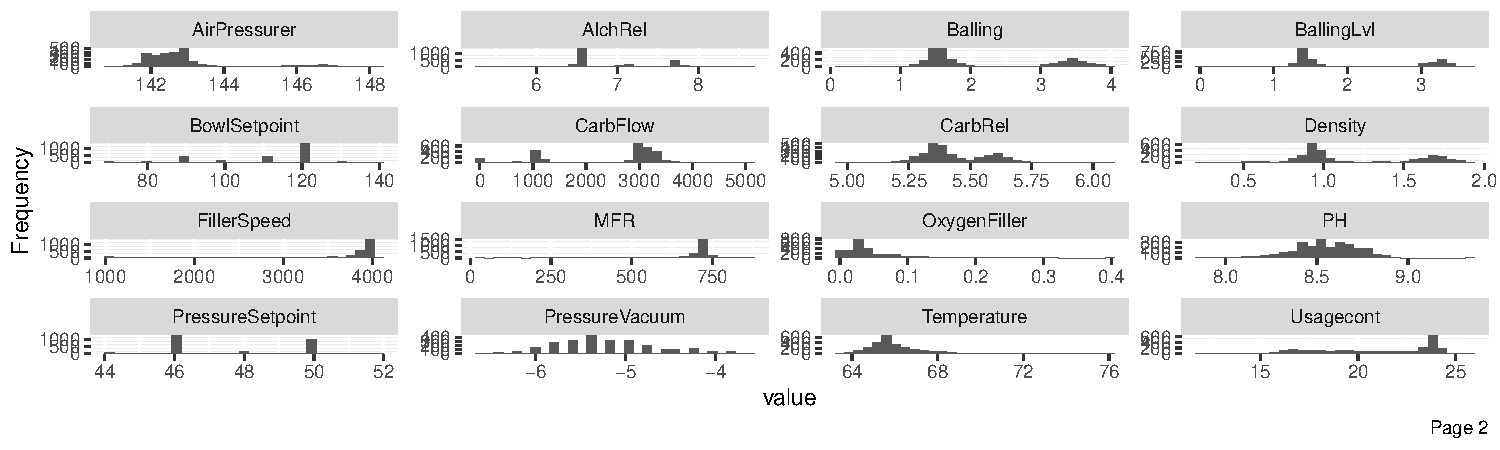
\includegraphics{Project2-VH_files/figure-latex/project2a4-2.pdf}

We observe evidence of outliers in addition to skew such as in the
varibales Temperature. Based on the information we have gathered from
our EDA, we can move into the data processing phase where we will
address our findings. We will not know the true effect of outliers until
we build and diagnose our models. We aniticipate linear model to perform
worse than NNET.

\newpage

\hypertarget{data-preperation}{%
\section{Data Preperation}\label{data-preperation}}

We will use the MICE method to impute missing variables. We will also
evaluate the which predictors have near zero variance. This will help us
identify pedictors that need to be dropped from the data frame all
together.We will hold off on removing predictors that have strong
pairwise correlation until after we see how it affects our models. Andy
has written code that nicely completes the data processing steps.

\begin{Shaded}
\begin{Highlighting}[]
\CommentTok{# set seed for split to allow for reproducibility}
\KeywordTok{set.seed}\NormalTok{(}\DecValTok{58677}\NormalTok{)}
\CommentTok{# use mice w/ default settings to impute missing data}
\NormalTok{miceImput <-}\StringTok{ }\KeywordTok{mice}\NormalTok{(df, }\DataTypeTok{printFlag =} \OtherTok{FALSE}\NormalTok{)}

\CommentTok{# add imputed data to original data set}
\NormalTok{df_mice <-}\StringTok{ }\NormalTok{mice}\OperatorTok{::}\KeywordTok{complete}\NormalTok{(miceImput)}
\NormalTok{df_mice}\OperatorTok{$}\NormalTok{BrandCode[}\KeywordTok{is.na}\NormalTok{(df_mice}\OperatorTok{$}\NormalTok{BrandCode)] <-}\StringTok{ "B"}

\NormalTok{zero_cols <-}\StringTok{ }\KeywordTok{nearZeroVar}\NormalTok{(df_mice)}
\NormalTok{df_final <-}\StringTok{ }\NormalTok{df_mice[, }\OperatorTok{-}\NormalTok{zero_cols]  }\CommentTok{# drop these zero variance columns }
\NormalTok{df_final}\OperatorTok{$}\NormalTok{BrandCode <-}\StringTok{ }\KeywordTok{as.factor}\NormalTok{(df_final}\OperatorTok{$}\NormalTok{BrandCode)}

\CommentTok{# convert categorical factor into numeric}
\NormalTok{M <-}\StringTok{ }\NormalTok{df_final}
\NormalTok{must_convert <-}\StringTok{ }\KeywordTok{sapply}\NormalTok{(M, is.factor)  }\CommentTok{# logical vector telling if a variable needs to be displayed as numeric}
\NormalTok{BrandNumeric <-}\StringTok{ }\KeywordTok{sapply}\NormalTok{(M[, must_convert], unclass)  }\CommentTok{# data.frame of all categorical variables now displayed as numeric}
\NormalTok{df_final2 <-}\StringTok{ }\KeywordTok{cbind}\NormalTok{(M[, }\OperatorTok{!}\NormalTok{must_convert], BrandNumeric)  }\CommentTok{# complete data.frame with all variables put together}

\CommentTok{# split data train/test}
\NormalTok{training <-}\StringTok{ }\NormalTok{df_final}\OperatorTok{$}\NormalTok{PH }\OperatorTok\StringTok{ }\KeywordTok{createDataPartition}\NormalTok{(}\DataTypeTok{p =} \FloatTok{0.8}\NormalTok{, }\DataTypeTok{list =} \OtherTok{FALSE}\NormalTok{)}
\NormalTok{df_train <-}\StringTok{ }\NormalTok{df_final[training, ]}
\NormalTok{df_test <-}\StringTok{ }\NormalTok{df_final[}\OperatorTok{-}\NormalTok{training, ]}
\end{Highlighting}
\end{Shaded}

\hypertarget{modeling}{%
\section{Modeling}\label{modeling}}

\hypertarget{linear-models}{%
\subsection{Linear Models}\label{linear-models}}

Linear Model: The first model we will be building is the classical
linear model. The linear model represents the taret variable as a
function of its predictor variables. Beta represents the linear
parameter estimate and epsilon represents the error term.
\(y={ \beta }_{ 0 }+\sum { { \beta }_{ i }{ X }_{ i }+{ \epsilon }_{ i } }\)

There are some assumptions that need to be followed regarding linear
regression. The first is that the residuals need to follow a near normal
distribution and the second is that variance has to be constant. We have
some diagnostic tests that can help us determine if these assumptions
are satisfied or not. These assumptions need to be checked before we
even consider taking into account how the model fits.

\begin{Shaded}
\begin{Highlighting}[]
\KeywordTok{par}\NormalTok{(}\DataTypeTok{mfrow =} \KeywordTok{c}\NormalTok{(}\DecValTok{2}\NormalTok{, }\DecValTok{2}\NormalTok{))}

\NormalTok{lm1 <-}\StringTok{ }\KeywordTok{lm}\NormalTok{(PH }\OperatorTok{~}\StringTok{ }\NormalTok{., }\DataTypeTok{data =}\NormalTok{ df_train)}

\CommentTok{# tab_model(lm1)}

\CommentTok{# summary(lm1)}

\CommentTok{# plot(lm1)}
\end{Highlighting}
\end{Shaded}

Lets examine some metrics against this model. The first is to compute
VIF numbers, also known as variance inflation numbers. The VIF numbers
will also provide direction into which variables to remove from future
iterations of the linear model. We typically remove predictors with a
VIF bigger than 4. In this case, we remove CarbPressurem CarbTemp,
Balling, AlchRel, and BallingLvl.
\url{https://www.researchgate.net/post/Multicollinearity_issues_is_a_value_less_than_10_acceptable_for_VIF}

\begin{Shaded}
\begin{Highlighting}[]
\KeywordTok{vif}\NormalTok{(lm1) }\OperatorTok\StringTok{ }\KeywordTok{kable}\NormalTok{(}\DataTypeTok{caption =} \StringTok{"Linear Model 1 Variance Inflation Numbers"}\NormalTok{) }\OperatorTok\StringTok{ }
\StringTok{    }\KeywordTok{kable_styling}\NormalTok{(}\DataTypeTok{full_width =}\NormalTok{ F, }\DataTypeTok{position =} \StringTok{"center"}\NormalTok{) }\OperatorTok\StringTok{ }\KeywordTok{row_spec}\NormalTok{()}
\end{Highlighting}
\end{Shaded}

\begin{table}[H]

\caption{\label{tab:project2a7}Linear Model 1 Variance Inflation Numbers}
\centering
\begin{tabular}[t]{l|r|r|r}
\hline
\textbf{ } & \textbf{GVIF} & \textbf{Df} & \textbf{GVIF\textasciicircum{}(1/(2*Df))}\\
\hline
\rowcolor{gray!6}  BrandCode & 53.571866 & 3 & 1.941584\\
\hline
CarbVolume & 13.634820 & 1 & 3.692536\\
\hline
\rowcolor{gray!6}  FillOunces & 1.160774 & 1 & 1.077392\\
\hline
PCVolume & 1.502752 & 1 & 1.225868\\
\hline
\rowcolor{gray!6}  CarbPressure & 32.477299 & 1 & 5.698886\\
\hline
CarbTemp & 26.671687 & 1 & 5.164464\\
\hline
\rowcolor{gray!6}  PSC & 1.153714 & 1 & 1.074111\\
\hline
PSCFill & 1.100332 & 1 & 1.048967\\
\hline
\rowcolor{gray!6}  PSCCO2 & 1.071535 & 1 & 1.035150\\
\hline
MnfFlow & 4.389162 & 1 & 2.095033\\
\hline
\rowcolor{gray!6}  CarbPressure1 & 1.572528 & 1 & 1.254005\\
\hline
FillPressure & 2.074542 & 1 & 1.440327\\
\hline
\rowcolor{gray!6}  HydPressure2 & 9.197523 & 1 & 3.032742\\
\hline
HydPressure3 & 12.507241 & 1 & 3.536558\\
\hline
\rowcolor{gray!6}  HydPressure4 & 2.650557 & 1 & 1.628053\\
\hline
FillerLevel & 11.055076 & 1 & 3.324918\\
\hline
\rowcolor{gray!6}  FillerSpeed & 11.544613 & 1 & 3.397737\\
\hline
Temperature & 1.400337 & 1 & 1.183358\\
\hline
\rowcolor{gray!6}  Usagecont & 1.703794 & 1 & 1.305295\\
\hline
CarbFlow & 2.356651 & 1 & 1.535139\\
\hline
\rowcolor{gray!6}  Density & 16.299332 & 1 & 4.037243\\
\hline
MFR & 9.832086 & 1 & 3.135616\\
\hline
\rowcolor{gray!6}  Balling & 71.779454 & 1 & 8.472276\\
\hline
PressureVacuum & 2.685955 & 1 & 1.638888\\
\hline
\rowcolor{gray!6}  OxygenFiller & 1.522703 & 1 & 1.233979\\
\hline
BowlSetpoint & 11.584124 & 1 & 3.403546\\
\hline
\rowcolor{gray!6}  PressureSetpoint & 2.268053 & 1 & 1.506006\\
\hline
AirPressurer & 1.184406 & 1 & 1.088304\\
\hline
\rowcolor{gray!6}  AlchRel & 23.237818 & 1 & 4.820562\\
\hline
CarbRel & 5.258863 & 1 & 2.293221\\
\hline
\rowcolor{gray!6}  BallingLvl & 54.441289 & 1 & 7.378434\\
\hline
\end{tabular}
\end{table}

We also want to see if outliers had any significant effect on our model
by performing a significance test using Bonferroni statistics. According
to our test, the low p value suggests that outliers are not significant
and we should not go through the effort to treat outliers.

\begin{Shaded}
\begin{Highlighting}[]
\KeywordTok{outlierTest}\NormalTok{(lm1)}
\end{Highlighting}
\end{Shaded}

\begin{verbatim}
     rstudent unadjusted p-value Bonferroni p
1093  5.85526         5.5454e-09   1.1396e-05
\end{verbatim}

We fit a new LM with features showing high VIF removed.

\begin{Shaded}
\begin{Highlighting}[]
\KeywordTok{par}\NormalTok{(}\DataTypeTok{mfrow =} \KeywordTok{c}\NormalTok{(}\DecValTok{2}\NormalTok{, }\DecValTok{2}\NormalTok{))}

\NormalTok{lm2 <-}\StringTok{ }\KeywordTok{lm}\NormalTok{(PH }\OperatorTok{~}\StringTok{ }\NormalTok{. }\OperatorTok{-}\StringTok{ }\NormalTok{BallingLvl }\OperatorTok{-}\StringTok{ }\NormalTok{AlchRel }\OperatorTok{-}\StringTok{ }\NormalTok{Balling }\OperatorTok{-}\StringTok{ }\NormalTok{CarbTemp }\OperatorTok{-}\StringTok{ }
\StringTok{    }\NormalTok{CarbPressure, }\DataTypeTok{data =}\NormalTok{ df_train)}

\CommentTok{# tab_model(lm2)}
\end{Highlighting}
\end{Shaded}

The adjusted r squared without the high VIF numbers remains
unchanged,hence we were able to simplify our model without a change in
data variability capture. We can furthur remove predictors by
calculating variable importance.

\begin{Shaded}
\begin{Highlighting}[]
\NormalTok{lm2_imp <-}\StringTok{ }\KeywordTok{varImp}\NormalTok{(lm2, }\DataTypeTok{scale =} \OtherTok{TRUE}\NormalTok{)}

\NormalTok{lm2_imp }\OperatorTok\StringTok{ }\KeywordTok{kable}\NormalTok{(}\DataTypeTok{caption =} \StringTok{"Linear Model 2 Variable Importance"}\NormalTok{) }\OperatorTok\StringTok{ }
\StringTok{    }\KeywordTok{kable_styling}\NormalTok{() }\OperatorTok\StringTok{ }\KeywordTok{row_spec}\NormalTok{()}
\end{Highlighting}
\end{Shaded}

\begin{table}[H]

\caption{\label{tab:project2a10}Linear Model 2 Variable Importance}
\centering
\begin{tabular}[t]{l|r}
\hline
\textbf{ } & \textbf{Overall}\\
\hline
\rowcolor{gray!6}  BrandCodeB & 0.6751499\\
\hline
BrandCodeC & 5.8589596\\
\hline
\rowcolor{gray!6}  BrandCodeD & 6.5503953\\
\hline
CarbVolume & 2.2600273\\
\hline
\rowcolor{gray!6}  FillOunces & 2.1716942\\
\hline
PCVolume & 1.5224876\\
\hline
\rowcolor{gray!6}  PSC & 1.5731511\\
\hline
PSCFill & 1.2302135\\
\hline
\rowcolor{gray!6}  PSCCO2 & 2.7008473\\
\hline
MnfFlow & 13.9429622\\
\hline
\rowcolor{gray!6}  CarbPressure1 & 7.5918084\\
\hline
FillPressure & 2.0097608\\
\hline
\rowcolor{gray!6}  HydPressure2 & 1.4157779\\
\hline
HydPressure3 & 4.6336202\\
\hline
\rowcolor{gray!6}  HydPressure4 & 0.7423533\\
\hline
FillerLevel & 1.9066804\\
\hline
\rowcolor{gray!6}  FillerSpeed & 2.6517876\\
\hline
Temperature & 6.2404708\\
\hline
\rowcolor{gray!6}  Usagecont & 5.7947060\\
\hline
CarbFlow & 1.6203759\\
\hline
\rowcolor{gray!6}  Density & 3.5540669\\
\hline
MFR & 3.5678464\\
\hline
\rowcolor{gray!6}  PressureVacuum & 0.1724955\\
\hline
OxygenFiller & 3.8880210\\
\hline
\rowcolor{gray!6}  BowlSetpoint & 4.7217460\\
\hline
PressureSetpoint & 4.3666264\\
\hline
\rowcolor{gray!6}  AirPressurer & 0.8192357\\
\hline
CarbRel & 2.8073009\\
\hline
\end{tabular}
\end{table}

\begin{Shaded}
\begin{Highlighting}[]
\CommentTok{# plot(lm2_imp)}
\end{Highlighting}
\end{Shaded}

BrandCode, PSCCO2, FillerSpeed, MFR,and PressureVacuum are flagged as
the least important variables. We will remove these from the overall
linear model and then compare how each of the three linear models does
against each other.

\begin{Shaded}
\begin{Highlighting}[]
\KeywordTok{par}\NormalTok{(}\DataTypeTok{mfrow =} \KeywordTok{c}\NormalTok{(}\DecValTok{2}\NormalTok{, }\DecValTok{2}\NormalTok{))}

\NormalTok{lm3 <-}\StringTok{ }\KeywordTok{lm}\NormalTok{(PH }\OperatorTok{~}\StringTok{ }\NormalTok{. }\OperatorTok{-}\StringTok{ }\NormalTok{BallingLvl }\OperatorTok{-}\StringTok{ }\NormalTok{AlchRel }\OperatorTok{-}\StringTok{ }\NormalTok{Balling }\OperatorTok{-}\StringTok{ }\NormalTok{BrandCode }\OperatorTok{-}\StringTok{ }
\StringTok{    }\NormalTok{CarbTemp }\OperatorTok{-}\StringTok{ }\NormalTok{CarbPressure }\OperatorTok{-}\StringTok{ }\NormalTok{PSCCO2 }\OperatorTok{-}\StringTok{ }\NormalTok{FillerSpeed }\OperatorTok{-}\StringTok{ }\NormalTok{MFR }\OperatorTok{-}\StringTok{ }\NormalTok{PressureVacuum, }
    \DataTypeTok{data =}\NormalTok{ df_train)}

\KeywordTok{tab_model}\NormalTok{(lm1, lm2, lm3)}
\end{Highlighting}
\end{Shaded}

~

PH

PH

PH

Predictors

Estimates

CI

p

Estimates

CI

p

Estimates

CI

p

(Intercept)

11.36

9.01~--~13.71

\textless0.001

11.32

9.42~--~13.22

\textless0.001

11.75

9.76~--~13.74

\textless0.001

BrandCode {[}B{]}

0.07

0.02~--~0.12

0.005

0.01

-0.02~--~0.05

0.500

BrandCode {[}C{]}

-0.07

-0.11~--~-0.02

0.007

-0.12

-0.16~--~-0.08

\textless0.001

BrandCode {[}D{]}

0.04

0.00~--~0.08

0.033

0.09

0.06~--~0.11

\textless0.001

CarbVolume

-0.15

-0.35~--~0.05

0.134

-0.12

-0.23~--~-0.02

0.024

0.02

-0.09~--~0.13

0.733

FillOunces

-0.08

-0.15~--~-0.02

0.017

-0.08

-0.15~--~-0.01

0.030

-0.13

-0.20~--~-0.06

0.001

PCVolume

-0.08

-0.20~--~0.03

0.145

-0.09

-0.20~--~0.03

0.128

-0.08

-0.20~--~0.04

0.193

CarbPressure

0.00

-0.00~--~0.01

0.364

CarbTemp

-0.00

-0.01~--~0.00

0.495

PSC

-0.11

-0.24~--~0.01

0.082

-0.10

-0.23~--~0.03

0.116

-0.13

-0.26~--~0.01

0.065

PSCFill

-0.03

-0.08~--~0.02

0.213

-0.03

-0.08~--~0.02

0.219

-0.06

-0.11~--~-0.00

0.035

PSCCO2

-0.17

-0.31~--~-0.03

0.015

-0.19

-0.33~--~-0.05

0.007

MnfFlow

-0.00

-0.00~--~-0.00

\textless0.001

-0.00

-0.00~--~-0.00

\textless0.001

-0.00

-0.00~--~-0.00

\textless0.001

CarbPressure1

0.01

0.00~--~0.01

\textless0.001

0.01

0.00~--~0.01

\textless0.001

0.01

0.00~--~0.01

\textless0.001

FillPressure

0.00

-0.00~--~0.00

0.091

0.00

0.00~--~0.01

0.045

0.00

-0.00~--~0.01

0.068

HydPressure2

-0.00

-0.00~--~0.00

0.163

-0.00

-0.00~--~0.00

0.157

-0.00

-0.00~--~0.00

0.076

HydPressure3

0.00

0.00~--~0.00

\textless0.001

0.00

0.00~--~0.00

\textless0.001

0.00

0.00~--~0.00

\textless0.001

HydPressure4

0.00

-0.00~--~0.00

0.673

0.00

-0.00~--~0.00

0.458

-0.00

-0.00~--~0.00

0.190

FillerLevel

-0.00

-0.00~--~0.00

0.058

-0.00

-0.00~--~0.00

0.057

-0.00

-0.00~--~0.00

0.265

FillerSpeed

0.00

0.00~--~0.00

0.003

0.00

0.00~--~0.00

0.008

Temperature

-0.01

-0.02~--~-0.01

\textless0.001

-0.02

-0.02~--~-0.01

\textless0.001

-0.02

-0.02~--~-0.01

\textless0.001

Usagecont

-0.01

-0.01~--~-0.00

\textless0.001

-0.01

-0.01~--~-0.00

\textless0.001

-0.01

-0.01~--~-0.01

\textless0.001

CarbFlow

0.00

-0.00~--~0.00

0.169

0.00

-0.00~--~0.00

0.105

0.00

-0.00~--~0.00

0.333

Density

-0.11

-0.17~--~-0.05

\textless0.001

-0.08

-0.13~--~-0.04

\textless0.001

-0.07

-0.10~--~-0.04

\textless0.001

MFR

-0.00

-0.00~--~-0.00

0.001

-0.00

-0.00~--~-0.00

\textless0.001

Balling

-0.10

-0.15~--~-0.04

\textless0.001

PressureVacuum

-0.02

-0.04~--~-0.00

0.017

-0.00

-0.02~--~0.01

0.863

OxygenFiller

-0.33

-0.49~--~-0.18

\textless0.001

-0.31

-0.47~--~-0.15

\textless0.001

-0.33

-0.50~--~-0.17

\textless0.001

BowlSetpoint

0.00

0.00~--~0.00

\textless0.001

0.00

0.00~--~0.00

\textless0.001

0.00

0.00~--~0.00

0.001

PressureSetpoint

-0.01

-0.01~--~-0.00

\textless0.001

-0.01

-0.01~--~-0.01

\textless0.001

-0.01

-0.02~--~-0.01

\textless0.001

AirPressurer

-0.00

-0.01~--~0.00

0.349

-0.00

-0.01~--~0.00

0.413

-0.00

-0.01~--~0.00

0.406

AlchRel

0.12

0.06~--~0.17

\textless0.001

CarbRel

0.03

-0.08~--~0.13

0.611

0.14

0.04~--~0.24

0.005

0.22

0.12~--~0.32

\textless0.001

BallingLvl

0.11

0.06~--~0.16

\textless0.001

Observations

2055

2055

2055

R2 / R2 adjusted

0.423 / 0.414

0.411 / 0.403

0.341 / 0.335

Across all three models, our adjusted R squared remains unchanged yet we
were able to simplify the model. Using lm3, we will now check if the
linear regression assumptions are satisfied.

\begin{Shaded}
\begin{Highlighting}[]
\KeywordTok{hist}\NormalTok{(lm3}\OperatorTok{$}\NormalTok{residuals)}
\end{Highlighting}
\end{Shaded}

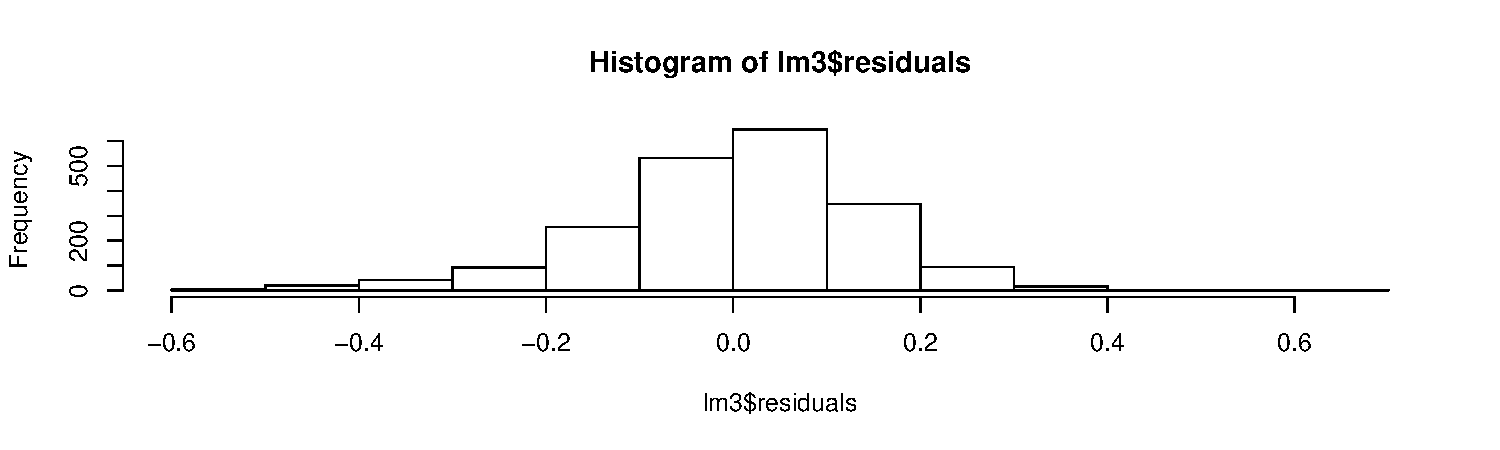
\includegraphics{Project2-VH_files/figure-latex/project2a12-1.pdf}

\begin{Shaded}
\begin{Highlighting}[]
\KeywordTok{qqnorm}\NormalTok{(lm3}\OperatorTok{$}\NormalTok{residuals)}
\KeywordTok{qqline}\NormalTok{(lm3}\OperatorTok{$}\NormalTok{residuals)}
\end{Highlighting}
\end{Shaded}

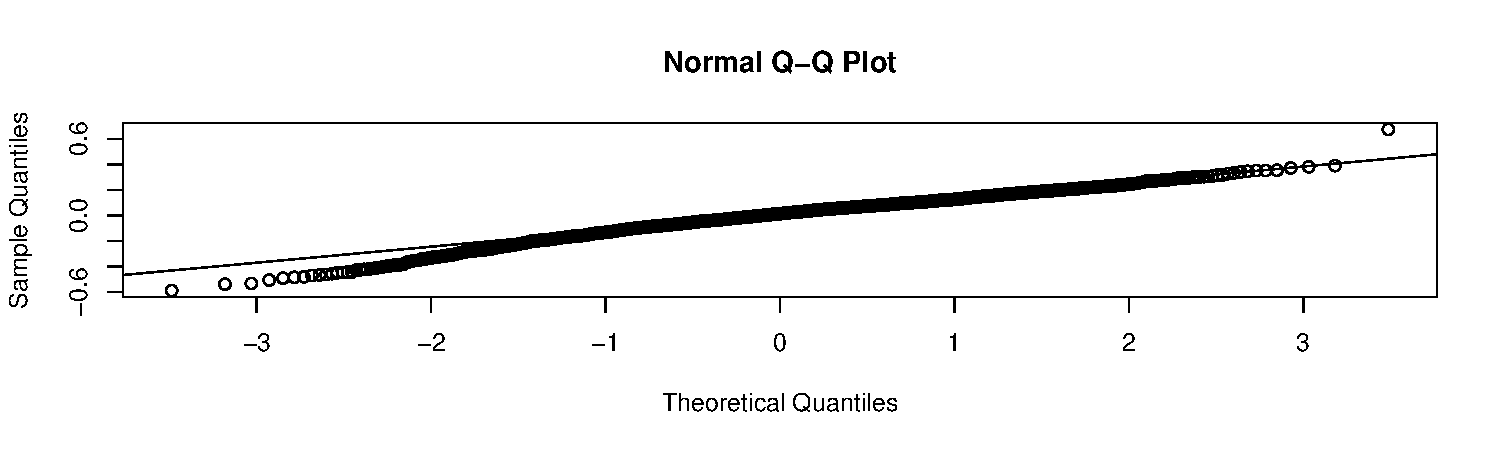
\includegraphics{Project2-VH_files/figure-latex/project2a12-2.pdf}

\begin{Shaded}
\begin{Highlighting}[]
\KeywordTok{plot}\NormalTok{(}\KeywordTok{fitted}\NormalTok{(lm3), }\KeywordTok{resid}\NormalTok{(lm3), }\DataTypeTok{col =} \StringTok{"dodgerblue"}\NormalTok{, }\DataTypeTok{pch =} \DecValTok{20}\NormalTok{, }\DataTypeTok{cex =} \FloatTok{1.5}\NormalTok{, }
    \DataTypeTok{xlab =} \StringTok{"Fitted"}\NormalTok{, }\DataTypeTok{ylab =} \StringTok{"Residuals"}\NormalTok{)}
\KeywordTok{abline}\NormalTok{(}\DataTypeTok{h =} \DecValTok{0}\NormalTok{, }\DataTypeTok{lty =} \DecValTok{2}\NormalTok{, }\DataTypeTok{col =} \StringTok{"darkorange"}\NormalTok{, }\DataTypeTok{lwd =} \DecValTok{2}\NormalTok{)}
\end{Highlighting}
\end{Shaded}

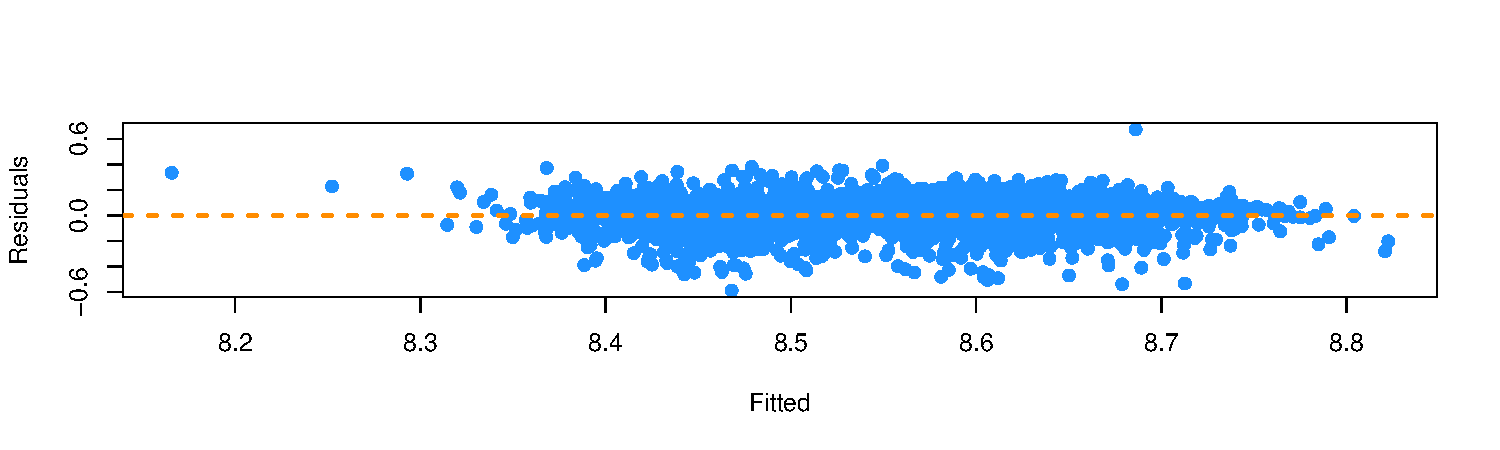
\includegraphics{Project2-VH_files/figure-latex/project2a12-3.pdf}

Our final LM seems to have near normal residuals and constant variance
as can be seen in the provided visualizations. We will stick to this
model to compare performance vs our NNEt model when we move into the
prediciton phase.

\hypertarget{model-2-nnet}{%
\subsection{Model 2: NNET}\label{model-2-nnet}}

\begin{Shaded}
\begin{Highlighting}[]
\KeywordTok{set.seed}\NormalTok{(}\DecValTok{58677}\NormalTok{)}

\CommentTok{# nn1<-nnet(PH~., data=df_train,size=2,linout=T)}

\CommentTok{# library(devtools)}
\CommentTok{# source_url('https://gist.githubusercontent.com/fawda123/7471137/raw/466c1474d0a505ff044412703516c34f1a4684a5/nnet#_plot_update.r')}

\NormalTok{nn_param <-}\StringTok{ }\KeywordTok{expand.grid}\NormalTok{(}\DataTypeTok{.size =} \KeywordTok{c}\NormalTok{(}\DecValTok{1}\OperatorTok{:}\DecValTok{10}\NormalTok{), }\DataTypeTok{.decay =} \KeywordTok{c}\NormalTok{(}\DecValTok{0}\NormalTok{, }\FloatTok{0.01}\NormalTok{, }
    \FloatTok{0.1}\NormalTok{))}

\NormalTok{nn1 <-}\StringTok{ }\KeywordTok{train}\NormalTok{(PH }\OperatorTok{~}\StringTok{ }\NormalTok{., }\DataTypeTok{data =}\NormalTok{ df_train, }\DataTypeTok{method =} \StringTok{"nnet"}\NormalTok{, }\DataTypeTok{maxit =} \DecValTok{1000}\NormalTok{, }
    \DataTypeTok{tuneGrid =}\NormalTok{ nn_param, }\DataTypeTok{trace =}\NormalTok{ F)}

\KeywordTok{print}\NormalTok{(nn1)}
\end{Highlighting}
\end{Shaded}

\begin{verbatim}
Neural Network 

2055 samples
  31 predictor

No pre-processing
Resampling: Bootstrapped (25 reps) 
Summary of sample sizes: 2055, 2055, 2055, 2055, 2055, 2055, ... 
Resampling results across tuning parameters:

  size  decay  RMSE      Rsquared     MAE     
   1    0.00   7.548907          NaN  7.546897
   1    0.01   7.548912  0.011144216  7.546902
   1    0.10   7.548941  0.003958879  7.546931
   2    0.00   7.548907          NaN  7.546897
   2    0.01   7.548910  0.001628368  7.546901
   2    0.10   7.548935  0.005394056  7.546926
   3    0.00   7.548907          NaN  7.546897
   3    0.01   7.548909  0.007667119  7.546900
   3    0.10   7.548925  0.008594149  7.546915
   4    0.00   7.548907          NaN  7.546897
   4    0.01   7.548909  0.004069893  7.546899
   4    0.10   7.548922  0.005327352  7.546912
   5    0.00   7.548907          NaN  7.546897
   5    0.01   7.548909  0.009582362  7.546899
   5    0.10   7.548919  0.006537257  7.546910
   6    0.00   7.548907          NaN  7.546897
   6    0.01   7.548908  0.006580751  7.546899
   6    0.10   7.548918  0.006370289  7.546908
   7    0.00   7.548907          NaN  7.546897
   7    0.01   7.548908  0.006409280  7.546899
   7    0.10   7.548916  0.006219754  7.546907
   8    0.00   7.548907          NaN  7.546897
   8    0.01   7.548908  0.003904651  7.546898
   8    0.10   7.548915  0.006191300  7.546906
   9    0.00   7.548907          NaN  7.546897
   9    0.01   7.548908  0.007235544  7.546898
   9    0.10   7.548915  0.005986394  7.546905
  10    0.00   7.548907          NaN  7.546897
  10    0.01   7.548908  0.006008687  7.546898
  10    0.10   7.548914  0.007989706  7.546905

RMSE was used to select the optimal model using the smallest value.
The final values used for the model were size = 1 and decay = 0.
\end{verbatim}

What were the most imporant features in our nnet model?

\begin{Shaded}
\begin{Highlighting}[]
\NormalTok{nn1_imp <-}\StringTok{ }\KeywordTok{varImp}\NormalTok{(nn1, }\DataTypeTok{scale =} \OtherTok{TRUE}\NormalTok{)}

\NormalTok{nn1_imp2 <-}\StringTok{ }\KeywordTok{as.data.frame}\NormalTok{(}\KeywordTok{as.matrix}\NormalTok{(nn1_imp}\OperatorTok{$}\NormalTok{importance))}

\CommentTok{# nn1_imp2%>% kable(caption='Linear Model 2 Variable}
\CommentTok{# Importance') %>% kable_styling() %>% row_spec()}

\KeywordTok{plot}\NormalTok{(nn1_imp)}
\end{Highlighting}
\end{Shaded}

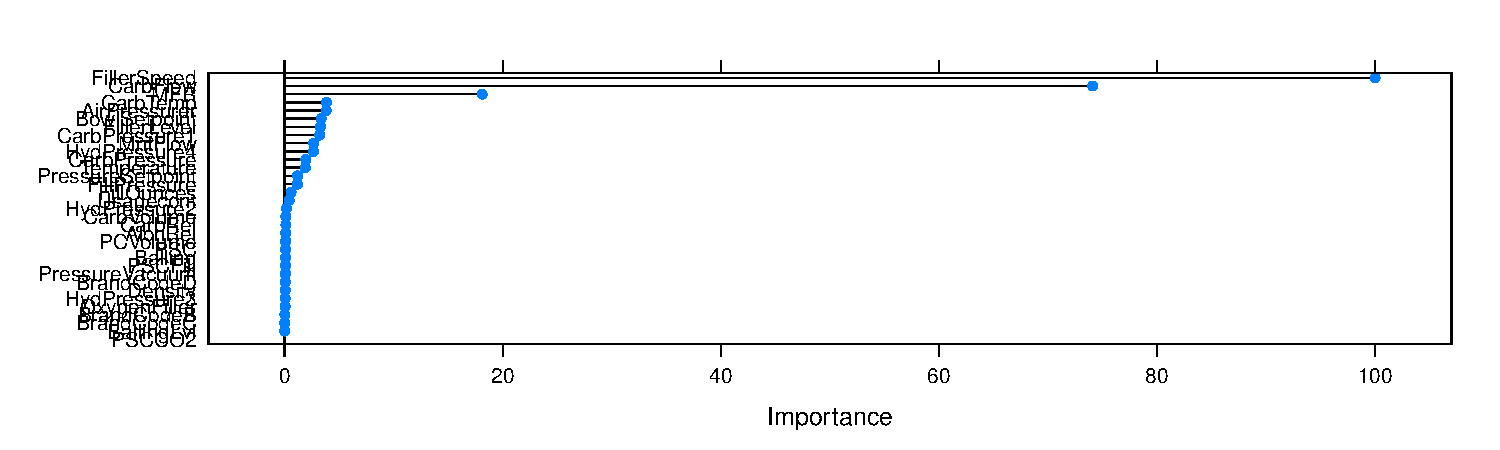
\includegraphics{Project2-VH_files/figure-latex/project2a14-1.pdf}

\hypertarget{mars-regression}{%
\subsection{MARS regression}\label{mars-regression}}

By experience, MARS has been one of the better performing models. We
should not spend too much time on trying to pick the best nnet model and
pick MARS as our third. We anticipate MARS to outperform LM and NNET.

\begin{Shaded}
\begin{Highlighting}[]
\CommentTok{# hyperparameter tuning for MARS}
\NormalTok{mars1 <-}\StringTok{ }\KeywordTok{earth}\NormalTok{(PH }\OperatorTok{~}\StringTok{ }\NormalTok{., }\DataTypeTok{data =}\NormalTok{ df_train)}

\KeywordTok{print}\NormalTok{(mars1)}
\end{Highlighting}
\end{Shaded}

\begin{verbatim}
Selected 18 of 22 terms, and 11 of 33 predictors
Termination condition: RSq changed by less than 0.001 at 22 terms
Importance: MnfFlow, BrandCodeC, AlchRel, PressureVacuum, Balling, ...
Number of terms at each degree of interaction: 1 17 (additive model)
GCV 0.01677669    RSS 33.31172    GRSq 0.4390952    RSq 0.4575109
\end{verbatim}

Baseline MARS model performed better than any of our NNET models or best
linear models.

\begin{Shaded}
\begin{Highlighting}[]
\NormalTok{mars_imp <-}\StringTok{ }\KeywordTok{varImp}\NormalTok{(mars1, }\DataTypeTok{scale =} \OtherTok{TRUE}\NormalTok{)}

\CommentTok{# mars_imp2<-as.data.frame(as.matrix(mars_imp$importance))}

\NormalTok{mars_imp }\OperatorTok\StringTok{ }\KeywordTok{kable}\NormalTok{(}\DataTypeTok{caption =} \StringTok{"Linear Model 2 Variable Importance"}\NormalTok{) }\OperatorTok\StringTok{ }
\StringTok{    }\KeywordTok{kable_styling}\NormalTok{()  }\CommentTok{# %>% row_spec()}
\end{Highlighting}
\end{Shaded}

\begin{table}[H]

\caption{\label{tab:project2a16}Linear Model 2 Variable Importance}
\centering
\begin{tabular}[t]{l|r}
\hline
  & Overall\\
\hline
\rowcolor{gray!6}  MnfFlow & 100.00000\\
\hline
BrandCodeC & 69.99661\\
\hline
\rowcolor{gray!6}  AlchRel & 56.69627\\
\hline
PressureVacuum & 52.13163\\
\hline
\rowcolor{gray!6}  Balling & 47.96692\\
\hline
Temperature & 41.15045\\
\hline
\rowcolor{gray!6}  Usagecont & 36.99494\\
\hline
CarbPressure1 & 31.91182\\
\hline
\rowcolor{gray!6}  BowlSetpoint & 28.07472\\
\hline
Density & 22.42714\\
\hline
\rowcolor{gray!6}  HydPressure3 & 18.32855\\
\hline
BrandCode & 0.00000\\
\hline
\rowcolor{gray!6}  CarbVolume & 0.00000\\
\hline
FillOunces & 0.00000\\
\hline
\rowcolor{gray!6}  PCVolume & 0.00000\\
\hline
CarbPressure & 0.00000\\
\hline
\rowcolor{gray!6}  CarbTemp & 0.00000\\
\hline
PSC & 0.00000\\
\hline
\rowcolor{gray!6}  PSCFill & 0.00000\\
\hline
PSCCO2 & 0.00000\\
\hline
\rowcolor{gray!6}  FillPressure & 0.00000\\
\hline
HydPressure2 & 0.00000\\
\hline
\rowcolor{gray!6}  HydPressure4 & 0.00000\\
\hline
FillerLevel & 0.00000\\
\hline
\rowcolor{gray!6}  FillerSpeed & 0.00000\\
\hline
CarbFlow & 0.00000\\
\hline
\rowcolor{gray!6}  MFR & 0.00000\\
\hline
OxygenFiller & 0.00000\\
\hline
\rowcolor{gray!6}  PressureSetpoint & 0.00000\\
\hline
AirPressurer & 0.00000\\
\hline
\rowcolor{gray!6}  CarbRel & 0.00000\\
\hline
BallingLvl & 0.00000\\
\hline
\end{tabular}
\end{table}

\begin{Shaded}
\begin{Highlighting}[]
\CommentTok{# plot(mars_imp2)}
\end{Highlighting}
\end{Shaded}

\begin{Shaded}
\begin{Highlighting}[]
\CommentTok{# hyperparameter tuning for MARS}
\NormalTok{mars2 <-}\StringTok{ }\KeywordTok{earth}\NormalTok{(PH }\OperatorTok{~}\StringTok{ }\NormalTok{BrandCode }\OperatorTok{+}\StringTok{ }\NormalTok{PressureVacuum }\OperatorTok{+}\StringTok{ }\NormalTok{AlchRel }\OperatorTok{+}\StringTok{ }\NormalTok{Balling }\OperatorTok{+}\StringTok{ }
\StringTok{    }\NormalTok{Temperature }\OperatorTok{+}\StringTok{ }\NormalTok{Usagecont }\OperatorTok{+}\StringTok{ }\NormalTok{CarbPressure1 }\OperatorTok{+}\StringTok{ }\NormalTok{BowlSetpoint }\OperatorTok{+}\StringTok{ }
\StringTok{    }\NormalTok{HydPressure3 }\OperatorTok{+}\StringTok{ }\NormalTok{Density, }\DataTypeTok{data =}\NormalTok{ df_train)}

\KeywordTok{print}\NormalTok{(mars2)}
\end{Highlighting}
\end{Shaded}

\begin{verbatim}
Selected 17 of 21 terms, and 9 of 12 predictors
Termination condition: Reached nk 25
Importance: Usagecont, BrandCodeC, BowlSetpoint, AlchRel, Balling, ...
Number of terms at each degree of interaction: 1 16 (additive model)
GCV 0.01781484    RSS 35.44315    GRSq 0.4043861    RSq 0.4228001
\end{verbatim}

\hypertarget{evaluation}{%
\section{Evaluation}\label{evaluation}}

\begin{Shaded}
\begin{Highlighting}[]
\CommentTok{# Make predictions}
\NormalTok{p1 <-}\StringTok{ }\NormalTok{lm3 }\OperatorTok\StringTok{ }\KeywordTok{predict}\NormalTok{(df_test)}
\NormalTok{p2 <-}\StringTok{ }\NormalTok{nn1 }\OperatorTok\StringTok{ }\KeywordTok{predict}\NormalTok{(df_test)}
\NormalTok{p3 <-}\StringTok{ }\NormalTok{mars2 }\OperatorTok\StringTok{ }\KeywordTok{predict}\NormalTok{(df_test)}

\CommentTok{# Model performance metrics}
\NormalTok{sum_t <-}\StringTok{ }\KeywordTok{data.frame}\NormalTok{(}
  \DataTypeTok{MODEL =} \KeywordTok{c}\NormalTok{(}\StringTok{'LinearModel'}\NormalTok{,}
            \StringTok{'NNET'}\NormalTok{,}
            \StringTok{'Mars'}\NormalTok{),}
  \DataTypeTok{RMSE =} \KeywordTok{c}\NormalTok{(caret}\OperatorTok{::}\KeywordTok{RMSE}\NormalTok{(p1, df_test}\OperatorTok{$}\NormalTok{PH),}
\NormalTok{           caret}\OperatorTok{::}\KeywordTok{RMSE}\NormalTok{(p2, df_test}\OperatorTok{$}\NormalTok{PH),}
\NormalTok{           caret}\OperatorTok{::}\KeywordTok{RMSE}\NormalTok{(p3, df_test}\OperatorTok{$}\NormalTok{PH)),}
      
  \DataTypeTok{Rsquare =} \KeywordTok{c}\NormalTok{(caret}\OperatorTok{::}\KeywordTok{R2}\NormalTok{(p1, df_test}\OperatorTok{$}\NormalTok{PH),}
\NormalTok{              caret}\OperatorTok{::}\KeywordTok{R2}\NormalTok{(p2, df_test}\OperatorTok{$}\NormalTok{PH),}
\NormalTok{              caret}\OperatorTok{::}\KeywordTok{R2}\NormalTok{(p3, df_test}\OperatorTok{$}\NormalTok{PH)),}
           
  \DataTypeTok{MAPE =} \KeywordTok{c}\NormalTok{(Metrics}\OperatorTok{::}\KeywordTok{mape}\NormalTok{(p1, df_test}\OperatorTok{$}\NormalTok{PH),}
\NormalTok{             Metrics}\OperatorTok{::}\KeywordTok{mape}\NormalTok{(p2, df_test}\OperatorTok{$}\NormalTok{PH),}
\NormalTok{             Metrics}\OperatorTok{::}\KeywordTok{mape}\NormalTok{(p3, df_test}\OperatorTok{$}\NormalTok{PH)))}
  
\NormalTok{sum_t}\OperatorTok\KeywordTok{kable}\NormalTok{(}\DataTypeTok{caption=}\StringTok{"Evaluation Summary on test set"}\NormalTok{, }\DataTypeTok{booktabs=}\NormalTok{T)}\OperatorTok\KeywordTok{kable_styling}\NormalTok{()}\OperatorTok\KeywordTok{row_spec}\NormalTok{()}
\end{Highlighting}
\end{Shaded}

\begin{table}[H]

\caption{\label{tab:project2a18}Evaluation Summary on test set}
\centering
\begin{tabular}[t]{lrrr}
\toprule
\textbf{MODEL} & \textbf{RMSE} & \textbf{Rsquare} & \textbf{MAPE}\\
\midrule
\rowcolor{gray!6}  LinearModel & 0.1395271 & 0.3352301 & 0.0126972\\
NNET & 7.5463897 & NA & 7.5444531\\
\rowcolor{gray!6}  Mars & 0.1332974 & 0.3923408 & 0.0121377\\
\bottomrule
\end{tabular}
\end{table}

As predicted MARS is the best of our three models.

\hypertarget{prediction}{%
\section{Prediction}\label{prediction}}

\begin{Shaded}
\begin{Highlighting}[]
\CommentTok{# remove space in-between variable names}
\KeywordTok{colnames}\NormalTok{(df_eval) <-}\StringTok{ }\KeywordTok{gsub}\NormalTok{(}\StringTok{" "}\NormalTok{, }\StringTok{""}\NormalTok{, }\KeywordTok{colnames}\NormalTok{(df_eval))}
\CommentTok{# remove column with zero-variance}
\KeywordTok{set.seed}\NormalTok{(}\DecValTok{58677}\NormalTok{)}
\CommentTok{# use mice w/ default settings to impute missing data}
\NormalTok{miceImput2 <-}\StringTok{ }\KeywordTok{mice}\NormalTok{(df_eval, }\DataTypeTok{printFlag =} \OtherTok{FALSE}\NormalTok{)}
\CommentTok{# add imputed data to original data set}
\NormalTok{df_mice2 <-}\StringTok{ }\NormalTok{mice}\OperatorTok{::}\KeywordTok{complete}\NormalTok{(miceImput2)}
\CommentTok{# table(df_eval$BrandCode, useNA = 'ifany')}
\NormalTok{df_mice2}\OperatorTok{$}\NormalTok{BrandCode[}\KeywordTok{is.na}\NormalTok{(df_mice2}\OperatorTok{$}\NormalTok{BrandCode)] <-}\StringTok{ "B"}
\CommentTok{# table(df_mice$BrandCode, useNA = 'ifany') Look for any}
\CommentTok{# features with no variance: zero_cols <- nearZeroVar(}
\CommentTok{# df_mice2 )}
\NormalTok{df_final22 <-}\StringTok{ }\NormalTok{df_mice2[, }\OperatorTok{-}\NormalTok{zero_cols]  }\CommentTok{# drop these zero variance columns }
\NormalTok{df_final22}\OperatorTok{$}\NormalTok{BrandCode <-}\StringTok{ }\KeywordTok{as.factor}\NormalTok{(df_final22}\OperatorTok{$}\NormalTok{BrandCode)}
\NormalTok{df_eval2 <-}\StringTok{ }\KeywordTok{subset}\NormalTok{(df_eval, }\DataTypeTok{select =} \OperatorTok{-}\NormalTok{PH)}
\NormalTok{pred_eval <-}\StringTok{ }\KeywordTok{predict}\NormalTok{(mars2, }\KeywordTok{subset}\NormalTok{(df_final22))}
\KeywordTok{write.csv}\NormalTok{(pred_eval, }\StringTok{"prediction.csv"}\NormalTok{)}
\end{Highlighting}
\end{Shaded}


\end{document}
